
\section{Modeling population dynamics and the diel vertical migration}
We apply our method to the diel vertical migration where the game is well-understood, but the interplay between the daily variations and the population dynamics have not been properly investigated. In addition  the Nash Equilibrium is known to be unique \citep{verticalmigration} at every instant.
We consider a food-chain in a water column, consisting of a resource $R$, a consumer $C$, and a predator $P$. The resource is thought of as phytoplankton, the consumer as copepods and the predator as forage fish. The predators and consumers are each distributed in the water column according to probability distributions, $\phi_c(z,t),\phi_p(z,t)$, and the resource is distributed according to $r(z,t)$.

%%See \Cref{fig:model_sketch}
%\begin{figure}
% \begin{centering}
%   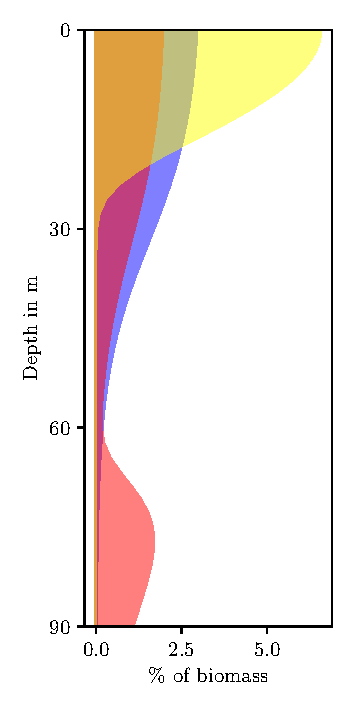
\includegraphics{plots/sketch_for_article.pdf}
% \end{centering}
% \label{fig:model_sketch}
% \caption{Sketch of model ecosystem, showing example distribution of resources, $(r(z,t)/R(t)$ \emph{(yellow)}, consumers ,$\phi_c$ \emph{(blue)} and predators, $\phi_p$ \emph{(red)}}
% \todo[inline]{Det er noget forvirrende at dette kun er ``example distribution''. Hvad skal læseren tage med sig fra denne figur?}
%\end{figure}

Forage fish are visual predators, so their predation success is heavily light dependent. The available light decreases with depth in the water column, and varies with the time of day.
The light intensity $I$ at depth $z$ is approximately $I(z) = I_0\exp(-kz)$, and the light-dependent clearance rate of a predator is $\beta_{p,0}$.  However, even when there is no light available there is still a chance of catching a consumer if it is directly encountered,  so the clearance rate, $\beta_p(z,t)$, of forage fish never goes to 0 even at the middle of the night or at the deepest depths.
\begin{equation*}
  \beta_p(z,t) = \beta_{p,0} \frac{I(z,t)}{1+I(z,t)} + \beta_{p,min}
\end{equation*}


We model the light-levels at the surface via. the python package pvlib \citep{holmgren2018pvlib} in the North Sea. The light levels are given by the direct horizontal light intensity at the sea-surface, neglecting more complicated optic effects. The model takes the precipitable water $w_a$, and aerosol optical depth, $aod$. We model light decay throughout the water column as $\exp(-kz)$.


In contrast to forage fish, copepods are olfactory predators, and their clearance rate, $\beta_c$, is essentially independent of depth and light levels.
\begin{align*}
	\beta_c(z,t) &=  \beta_{c,0}
\end{align*}

The interactions between the consumer and resource are local, as are the interactions between a predator and a consumer. The local encounter rate between consumers and resources is given by $C\beta_c(z,t)\phi_c(z,t)r(z,t)$, and the local encounter rate between predators and consumers is $CP\beta_p(z,t)\phi_c(z,t)\phi_p(z,t)$.

\subsection{Population dynamics}

The resource cannot move actively, so its time dynamics are naturally specified locally. The growth of the resource is modeled with a logistic growth, with a loss from grazing by consumers and diffusion from the natural movement of the water. We assume interactions can be described with a Type I functional response, allowing us to eventually use the method developed in \Cref{sec:gen_model}. The resource dynamics become:
\begin{equation}
  \label{eq:res_dyn}
	\dot{r} = r(z,t)\pa{1-\frac{r(z,t)}{r_{max}(z)}} - \beta_c(z,t)\phi_c(z,t)C(t) r(z,t)  + k \partial_z^2 r(z,t) \\
\end{equation}
%In natural environments, undersaturation of nutrients is the norm, \citep{}.

The total population growth of the consumer population is found by integrating the local grazing rate over the entire water column multiplied by a conversion efficiency $\epsilon$, subtracting the loss from predation. The growth of the predators is given by the predation rate integrated over the water column. The instantaneous pr. capita fitness of the consumer $F_c$ and predator $F_p$ without metabolic losses become:
\begin{equation}
  \begin{split}
	F_c(\phi_c, \phi_p) &= \int_0^{z_0} \varepsilon \beta_c(z,t)\phi_c(z,t)r(z,t) dz\\ &- P(t)\int_0^{z_0} \beta_p(z,t) \phi_c(z,t) \phi_p(z,t)dz \\
	F_p(\phi_c, \phi_p) &=  C(t) \int_0^{z_0} \varepsilon \beta_p(z,t)\phi_c(z,t)\phi_p(z,t) dz
  \end{split}
  \label{eq:fitness}
\end{equation}


Using \Cref{eq:fitness} we arrive at equations for the predator-prey population dynamics:
\begin{equation}
  \begin{split}
	\dot{C} &= C(t)\left ( F_c - \mu_C \right ) \\
	\dot{P} &= P(t) \left ( F_p - \mu_P  \right )
\end{split}
  \label{eq:population_growth_prob_dens}
\end{equation}

\subsection{Simulating the model}

%The instantaneous fitness pr. capita of a forage fish $(F_p)$ or copepod $(F_c)$ is given by t. We arrive at the fitness by dividing the population growth rate \Cref{eq:population_growth_prob_dens} by the total populations, eliminating the terms $C(t), P(t)$ outside the parentheses in \Cref{eq:population_growth_prob_dens}.

%\todo[inline]{Fitness er ikke det samme som specifikke vækstrater. }

%\todo[inline]{Når nu disse størrelser er indført, hvorfor så ikke bruge dem over det hele? Så ville mange formler være meget mere kompakte.}

At any instant, all consumers and predators simultaneously seek to find the strategy that maximizes their fitness ($F_c, F_p$) \Cref{eq:utility}. A strategy in our case is a square-integrable probability distribution in the water column, i.e. an element in $K$, \Cref{eq:space_of_dists}.

%The optimal strategy $\phi_c^*$ of a consumer depends on the strategy of the predators, and likewise for $\phi_p^*$ for the predators. the space of square-integrable probability distributions on $[0,z_0]$ by $K$ (\Cref{eq:space_of_dists}), this can be expressed as:
%\begin{align*}
%	\phi_c^*(z,t)(\phi_p) &= \argmax_{\phi_c \in K}  F_c(\phi_c, \phi_p)  \\
%	\phi_p^*(z,t)(\phi_c) &= \argmax_{\phi_p \in K} F_p(\phi_c, \phi_p)
%\end{align*}
Using the notation of \Cref{sec:gen_model}, with $F_i$ taking the place of $U_i$, the Nash equilibrium of the instantaneous game is:
\begin{equation}
  \label{eq:nash_equilibria}
  \begin{split}
  	\phi_c^{*,NE} &=  \argmax_{\phi_c \in K}  F_c(\phi_c, \phi_p^{*,NE}) \\
  	\phi_p^{*,NE} &=  \argmax_{\phi_p \in K} F_p(\phi_c^{*,NE}, \phi_p)
  \end{split}
\end{equation}
We apply the method \Cref{eq:lcp} to find the Nash equilibrium of the discretized system. Using the Nash equillibrium \Cref{eq:nash_equilibria} we are able to solve the time-dynamics for the predator-prey system \Cref{eq:population_growth_prob_dens} by a Euler scheme. The dynamics of the resource are more complicated due to the diffusion term, \Cref{eq:res_dyn}. We solve the partial differential equation for the resource using the method of exponential time-differencing \citep{hochbruck2010exponential} with a first-order approximation of the integral. Using exponential time-differencing guarantees a stable solution, though the system may be stiff \cite{hochbruck2010exponential}.

\subsection{Model parameters}
Following \citep{yodzis1992body}, we parameterize the clearance and loss rates in a metabolically scaled manner following Kleiber's law, \citep{yodzis1992body}, using scaling constants from \citep{kha_2019}. We use the default parameters in the clear-sky model, modeling a sequence of moonless nights. This is a bit of a simplification, but it should not have a great effect on our results. The North Sea is modeled with a rather high attenuation coefficient. We use the notation $\mathcal{N}(0,\sigma^2)$ for the normal distribution with mean $0$ and variance $\sigma^2$.


\begin{tabular}{l  l  l}
  Precipitable water & $w_a$ & 1 g $\cdot$ m$^{-3}$\\
  Aeorosol optical depth & $aod$ & 0.1 \\
  Light decay & $k$ & 0.1 m$^{-1}$\\
  Ocean depth & $z_0$ & 90 m \\
  Consumer mass & $m_c$ & 0.05 $g$ \\
  Predator mass & $m_p$ & 20 $g$ \\
  Consumer clearance rate & $\beta_c$ & 32 m$^{3}$ year$^{-1}$ \\
  Predator clearance rate & $\beta_p$ & 2800 m$^3$ year$^{-1}$ \\
  Consumer metabolic rate & $\mu_c$ & 0.24 g$^{3}$ year$^{-1}$ \\
  Predator metabolic rate & $\mu_p$ & 21 g$^3$ year$^{-1}$ \\
  Minimal attack rate & $\beta_0$ & $5 \cdot 10^{-3} \beta_p$ \\
  Phytoplankton growth & $\lambda$ & 100 year$^{-1}$ \\
  Phytoplankton max & $r_{max}$ & $10\mathcal{N}(0,6)$ g m $^{-1}$ \\
  Irrationality & $\sigma$ & 10 m$^2$ \\
  Diffusion rate & k & 500 m$^{2}$ year$^{-1}$ \\
  Initial consumers & $C_0$ & 4  g m$^{-2}$ \\
  Initial predators & $C_0$ & 0.04  g m$^{-2}$ \\
  Initial resources & $r_0$ & 4$\mathcal{N}(0,6)$ g m$^{-1}$
\end{tabular}

%%% Local Variables:
%%% mode: latex
%%% TeX-master: "main"
%%% End:
